Semiconductor laser -- knowledge from Condensed Matter Physics can be very useful here.

\begin{parts}
	\part
	\begin{figure}[H]
		\centering
		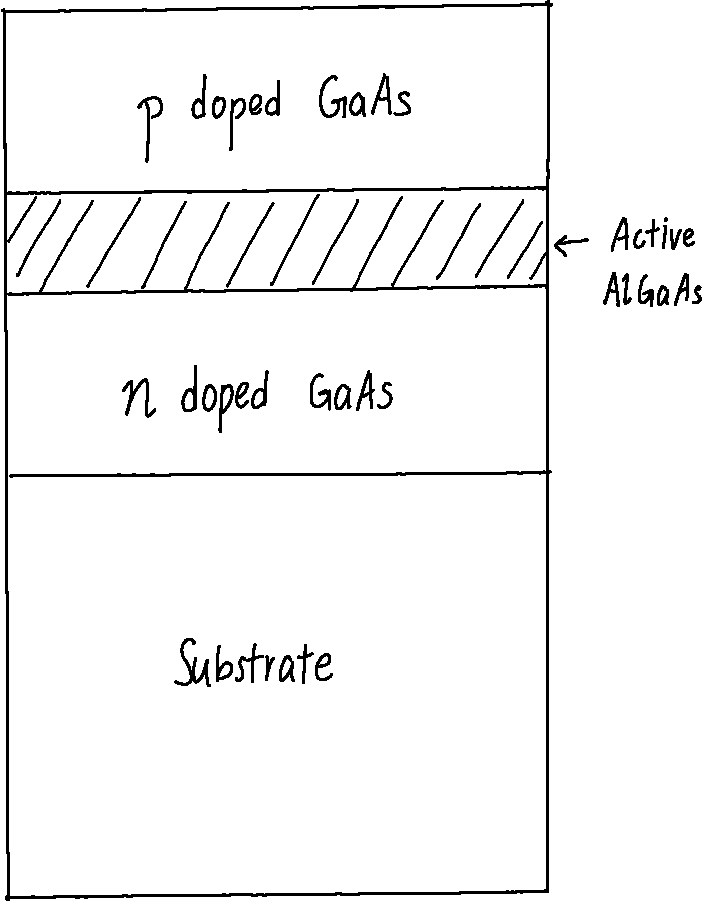
\includegraphics[width=.45\linewidth]{q1-double-heterostructure}
	\end{figure}
	A double heterostructure is a sandwich of p and n doped substance with much higher bandgap than the active region.
	This is useful in low threshold laser due to the good confinement of charge carriers, photon, and low leakage.
	
	\begin{figure}[H]
		\centering
		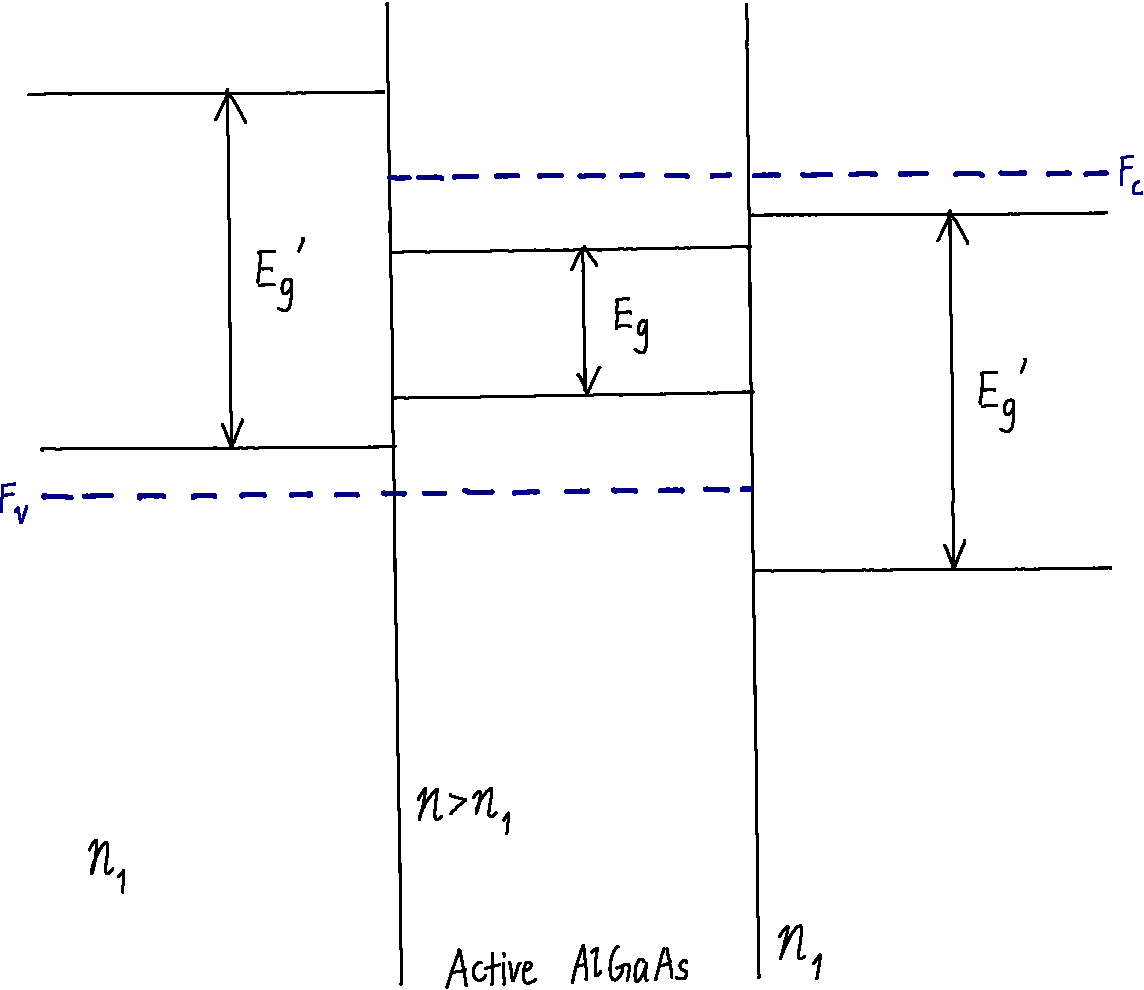
\includegraphics[width=.65\linewidth]{q1-energy}
	\end{figure}
	Note the separation of bandgap $\rightarrow$ charge carrier confined and little absorption for escaped beam.
	Also the refractive indices are such that the active region forms a waveguide.
	
	\part Quasi-Fermi energies are chemical potentials of the conduction/valence band in a local equilibrium.
	This is useful for lasing as pumping lasing means that the band population will be altered to a new and dynamic equilibrium than the static case.
	
	\part The gain coefficient is dependent on the joint density of states of transitions, together with the probability of net emission:
	\begin{align*}
		E_\textnormal{transition} &= E_1 - E_2 \\
		&= E_g + \frac{\hbar^2 k^2}{2\mu} \\
		&= \hbar\omega \\
		\frac{\hbar^2 k^2}{2\mu} &= \hbar\omega - E_g
	\end{align*}
	where $\mu^{-1} = m_e^{-1} + m_h^{-1}$ is the reduced mass of an electron-hole pair.
	
	Assuming isotropy, we have the following density of states:
	\begin{gather*}
		g(k) \inftsml{k} \propto k^2 \inftsml{k} \\
		\Rightarrow g(E) \inftsml{E} \propto \rbracket{\hbar\omega - E_g}^{1/2} \inftsml{E} \mtext{since $k \inftsml{k} \propto \inftsml{E}$}
	\end{gather*}
	
	Probability of emission: $f_c(E_1) \sbracket{1-f_v(E_2)}$
	
	Probability of absorption: $f_v(E_2) \sbracket{1-f_c(E_1)}$
	
	Hence probability of net emission:
	\begin{equation*}
		P(\textnormal{emission}) - P(\textnormal{absorption}) = f_c(E_1) - f_v(E_2)
	\end{equation*}
	
	As $\omega$ increases, gain increases as the d.o.s. of allowed transitions grows.
	Note that for temperature, the dependence has an optimal window as both $f_c$ and $f_v$ have the same limit as $T \rightarrow 0$ or $T \rightarrow \infty$, this is due to the fact that transitions in a semiconductor is a dynamic equilibrium.
	
	\part We want $\textnormal{gain} > 0$:
	\begin{align*}
		\Rightarrow f_c &> f_v \\
		\mathrm{e}^{(E_2 - F_v)/\boltzmann T} + 1 &> \mathrm{e}^{(E_1 - F_c)/\boltzmann T} + 1 \\
		\Rightarrow E_2 - F_v &> E_1 - F_c \\
		E_1 - E_2 &< F_c - F_v
	\end{align*}
	
	From above we also have $E_1 - E_2 = E_g + \hbar^2 k^2/2\mu > E_g$ hence the inequality.
	
	At $T = \SI{0}{\kelvin}$, we have:
	\begin{align*}
		f_c &\rightarrow \begin{cases}
			1 \hspace{1em} E_1 < F_c \\
			0 \hspace{1em} E_1 > F_c
		\end{cases} \\
		f_v &\rightarrow \begin{cases}
			1 \hspace{1em} E_2 < F_v \\
			0 \hspace{1em} E_2 > F_v
		\end{cases}
	\end{align*}
	
	But since $E_1 - E_2 < F_c - F_v$, we won't have $f_c = 1$ and $f_v = 0$ for all $\omega$, which leads to zero gain.
	\begin{figure}[H]
		\centering
		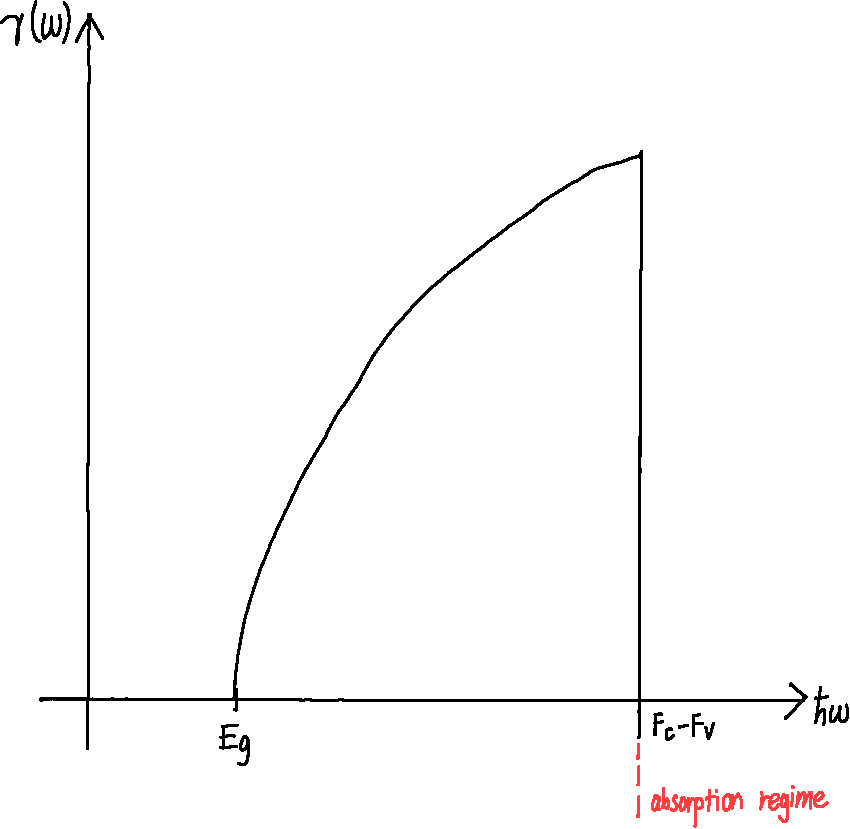
\includegraphics[width=.7\linewidth]{q1-gain-t0}
	\end{figure}
	
	At $T > \SI{0}{\kelvin}$, provided $E_1 - E_2 < F_c - F_v$, we have $f_c - f_v > 0$ and the limiting factor is the d.o.s. -- the gain begins at $\hbar\omega = E_g$ and grows before dropping to $0$ as $f_c - f_v \rightarrow 0$.
	\begin{figure}[H]
		\centering
		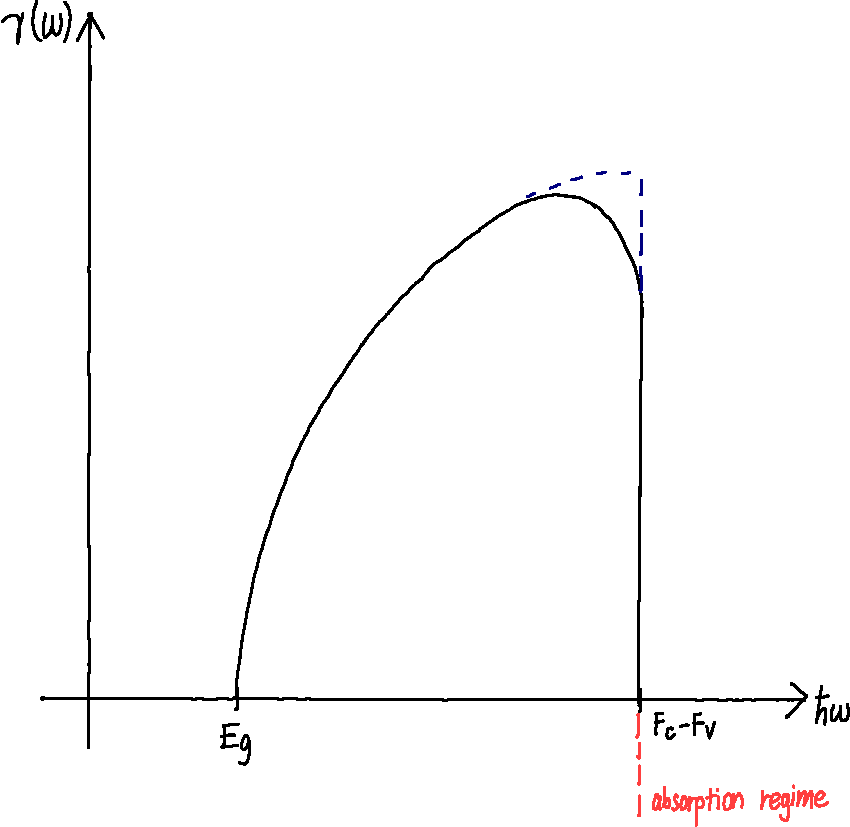
\includegraphics[width=.7\linewidth]{q1-gain-t}
	\end{figure}
	
	\part From the given electron density, we find:
	\begin{equation*}
		F_c = \frac{\hbar^2}{2m_e} \rbracket{N \cdot 3\pi^2}^{2/3} + E_g = \SI{1.78}{\electronvolt}
	\end{equation*}
	
	Similarly for holes:
	\begin{align*}
		N_\textnormal{hole} &= \frac{1}{3\pi^2} \rbracket{\frac{2m_h F_v}{\hbar^2}}^{3/2} \\
		\Rightarrow F_v &= \frac{\hbar^2}{2m_h} \rbracket{N_\textnormal{hole} \cdot 3\pi^2}^{2/3} = \SI{0.03}{\electronvolt}
	\end{align*}
	
	So $F_c - F_v = \SI{1.75}{\electronvolt} > E_g = \SI{1.54}{\electronvolt}$ is verified.
	
	Peak gain should occur when $E_1 - E_2$ is maximised, i.e. $F_c - F_v = \hbar kc = hc/\lambda$:
	\begin{equation*}
		\Rightarrow \lambda = \frac{hc}{F_c - F_v} = \SI{781}{\nano\metre}
	\end{equation*}
\end{parts}